\documentclass[../../../main.tex]{subfiles}
\begin{document}
On considère un ensemble fini $E$. Comme $E$ est fini, il est en bijection avec $\{0, \dots, n - 1\}$ où $n = |E|$. On cherche ici un moyen efficace de stocker et de manipuler une partition de $E$, c'est-à-dire une partition de $\{0, \dots, n-1\}$.

La manipulation de partitions de $E$ correspond exactement à la manipulation de classes d'équivalence de $E$. Les classes d'équivalences sont la conséquence d'une forme de clôture de relation entre objets (clôture réflexive-transitive-symétrique de la relation). Le lien direct avec les relations justifie théoriquement la manipulation des partitions d'ensembles par la manipulation de relations. L'efficacité remarquable des algorithmes qui en découlent en est une justification pratique.
\subsection{Signature}
\label{sub:partition_principe_et_signature}
L'objectif est principalement de travailler sur les classes d'équivalences d'une relation sur un ensemble, c'est-à-dire :
\begin{itemize}
	\item construire des classes d'équivalence d'un ensemble par unions itérés de classes au départ unitaires (ne contenant qu'un seul élément)
	\item trouver la classe d'équivalence d'un élément quelconque de l'ensemble (\textit{i.e.} son représentant)
	\item déterminer efficacement le nombre de classes d'équivalences dans l'ensemble par la relation
\end{itemize}
On en déduit la signature du type abstrait \textit{Partition} :

\textit{Partition} utilise \textit{Booléen}, \textit{Entier}
\begin{itemize}
	\item $creer(n:Entier)\rightarrow Partition$ renvoie une partition d'un ensemble à $n$ éléments en $n$ classes d'équivalences où chaque élément de l'ensemble est représentant de sa propre classe d'équivalence d'un seul élément.
	\item $unir(Partition, a:Entier, b:Entier)\rightarrow Partition$ renvoie la partition de $E$ où les classes d'équivalence de $\dot{a}$ et $\dot{b}$ sont unies en une seule classe d'équivalence
	\item $trouver(Partition, i:Entier)\rightarrow Entier$ renvoie $\dot{i}$ le représentant de la classe d'équivalence de $i$
	\item $nombre\_classes(Partition)\rightarrow Entier$ renvoie le nombre de classes d'équivalences de la partition.
\end{itemize}
\subsection{Principe sur un exemple naïf}
Prenons l'ensemble $E = \{0, 1, 2, 3, 4, 5\}$. Sa partition la plus fine est constituée de $6$ classes $P = \{\{0\}, \dots, \{5\}\}$. Si $\rightarrow$ est la relation (homogène sur $E$) associée à $P$, on a : $$\rightarrow = \{(0, 0), (1, 1), (2, 2), (3, 3), (4, 4), (5, 5)\}$$
représentée graphiquement par :
\begin{center}
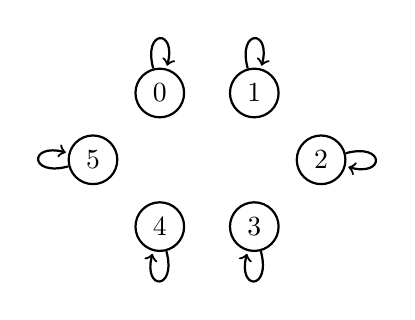
\begin{tikzpicture}[node distance={12mm}, thick, main/.style = {draw, circle}, auto=left] 
	% Sommets :
	\node[main] (0) {0}; 
	\node[main] (1) [right of=0] {1};
	\node[main] (2) [below right of=1] {2};
	\node[main] (3) [below left of=2] {3};
	\node[main] (5) [below left of=0] {5};
	\node[main] (4) [below right of=5] {4};
	% Arêtes
	\path
		(0) edge[loop above] (0)
		(1) edge[loop above] (1)
		(2) edge[loop right] (2)
		(3) edge[loop below] (3)
		(4) edge[loop below] (4)
		(5) edge[loop left] (5);
\end{tikzpicture}
\captionof{figure}{Graphe initial de la relation\label{graph:uf_init}}
\end{center}
On peut faire subir quelques transformations à $P$ selon les routines de manipulation décrites par la signature de \textit{Partition} :
\begin{itemize}
	\item $P\leftarrow unir(P, 0, 4) = \{\{0, 4\}, \{1\}, \{2\}, \{3\}, \{5\}\}$
	\item $P\leftarrow unir(P, 5, 1) = \{\{0, 4\}, \{1, 5\}, \{2\}, \{3\}\}$
	\item $trouver(P, 5) \rightarrow 1$
	\item $P \leftarrow unir(P, 5, 4) = unir(P, 1, 4) = \{\{0, 4, 1, 5\}, \{2\}, \{3\}\}$
	\item $trouver(P, 1) \rightarrow 4$
\end{itemize}
À la fin, on a $0\equiv 1\equiv 4\equiv 5$ dans $P$.

\textbf{Lien avec les relations et représentation graphique :} l'évolution de la partition peut être représentée par une relation $\rightarrow$ telle que pour toute classe $C$ de $E$, $e, f\in C \Leftrightarrow e\rightarrow^\star f$.

\begin{minipage}{0.49\textwidth}
\begin{center}
	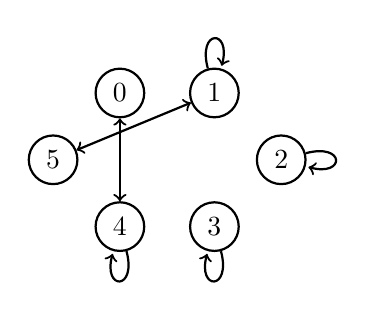
\begin{tikzpicture}[node distance={12mm}, thick, main/.style = {draw, circle}, auto=left] 
	% Sommets :
	\node[main] (0) {0}; 
	\node[main] (1) [right of=0] {1};
	\node[main] (2) [below right of=1] {2};
	\node[main] (3) [below left of=2] {3};
	\node[main] (5) [below left of=0] {5};
	\node[main] (4) [below right of=5] {4};
	% Arêtes
	\path
		(1) edge[loop above] (1)
		(2) edge[loop right] (2)
		(3) edge[loop below] (3)
		(4) edge[loop below] (4)
		(5) edge[<->] (1)
		(0) edge[<->] (4);
	\end{tikzpicture}
	\end{center}
\end{minipage}
\begin{minipage}{0.49\textwidth}
	\begin{center}
	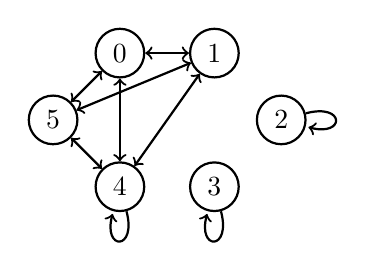
\begin{tikzpicture}[node distance={12mm}, thick, main/.style = {draw, circle}, auto=left] 
	% Sommets :
	\node[main] (0) {0}; 
	\node[main] (1) [right of=0] {1};
	\node[main] (2) [below right of=1] {2};
	\node[main] (3) [below left of=2] {3};
	\node[main] (5) [below left of=0] {5};
	\node[main] (4) [below right of=5] {4};
	% Arêtes
	\path
		(1) edge[<->] (4)
		(2) edge[loop right] (2)
		(3) edge[loop below] (3)
		(4) edge[loop below] (4)
		(5) edge[<->] (1)
		(5) edge[<->] (4)
		(5) edge[<->] (0)
		(0) edge[<->] (4)
		(0) edge[<->] (1);
	\end{tikzpicture}
	\end{center}
\end{minipage}

\begin{minipage}{0.5\textwidth}
\centering \captionof{figure}{Graphe après deux unions\label{graph:uf_deux_unions}}
\end{minipage}
\begin{minipage}{0.5\textwidth}
\centering \captionof{figure}{Graphe final après \textit{une} union\label{graph:uf_final}}
\end{minipage}

La partition représentée est simplement la clôture réflexive-transitive-symétrique du graphe final (après avoir subi toutes les unions).

\textbf{Problème de cette représentation \textit{naïve} :} en deux points :
\begin{itemize}
	\item Il est malheureusement très coûteux calculatoirement de \textit{maintenir} une relation d'équivalence lors de la modification de celle-ci. Par exemple, l'union de deux classes d'équivalences requiert de mettre en relation chacun des éléments de la première classe avec chacun des éléments de la seconde. Ainsi, l'union de deux classes d'équivalences $E_1$ et $E_2$ d'un ensemble $E$ nécessite $Card(E_1)\times Card(E_2)$ opérations.
	\item Par ailleurs, les classes d'équivalences de la relation font que chaque élément d'une partie de $E$ est représentant de cette partie. On ne peut pas utiliser ce critère de représentation pour vérifier que deux éléments $e_1$ et $e_2$ appartiennent à la même classe. Il faut à la place trouver ou non un chemin entre $e_1$ et $e_2$ dans le graphe, ce qui est également coûteux.
\end{itemize}
Finalement, cette représentation naïve est extrêmement coûteuse calculatoirement et ne permet pas d'implanter efficacement les deux opérations \textit{unir} et \textit{trouver}.
\subsection{La clef vers l'optimisation}
On observe que tous éléments d'une classe d'équivalence $C$ représentent cette classe. Si on choisit en revanche un \textit{unique} élément $r_C\in C$ pour représenter $C$, il faut simplement pour trouver la classe d'un élément $e\in E$ lui associer son représentant par un chemin d'arcs. Cette association fournit une nouvelle relation, noté $\rightarrow_r$ telle que :
$$\forall C\in (E/\rightarrow), \forall e\in E, \left(e\in C\Leftrightarrow \exists! e_1, \dots, e_{n-1}\in C\setminus\{r_C\}, e\rightarrow_r e_1 \rightarrow_r\dots \rightarrow_r e_{n-1}\rightarrow_r  r_C\right)$$
\textbf{En français :} un élément $e$ appartient à une classe d'équivalence définit par $\rightarrow$ si et seulement si il existe un unique chemin de $e$ vers $r_C$ définit par $\rightarrow_r$. $\rightarrow_r$ restreint donc $\rightarrow$ en ne conservant qu'un seul chemin de tout élément d'une classe vers son représentant. C'est-à-dire que $\rightarrow_r$ définit un arbre sur chaque classe $C$ dont la racine est $r_C$ (voir l'\refexercise{Arbres et graphes}).

\textbf{Remarques :}
\begin{itemize}
	\item cette définition de $\rightarrow_r$ n'assure absolument pas son unicité
	\item $\rightarrow$ est exactement la clôture réflexive-transitive-symétrique de $\rightarrow_r$, ce qui montre que $\rightarrow_r$ désigne le même quotient (après clôture de la relation)
	\item la relation $\rightarrow_r$ est fonctionnelle : chaque élément ne peut se déplacer que vers un unique autre élément dans le graphe (dans le cas contraire, le chemin vers $r_C$ n'est pas unique). Autrement dit, pour tout $s\in E, d_{\rightarrow_r}^{+}(s) = 1$ ($d_{\rightarrow_r}^+$ est le degré \textit{sortant} de $s$ dans le graphe représentatif de la relation $\rightarrow_r$).
\end{itemize}

\subsubsection{Caractérisation relationnelle des opérations ``unir'' et ``trouver''}
De la définition et des remarques précédentes on déduit qu'étant donné un élément $e\in E$, on peut trouver sa classe d'équivalence par $\rightarrow$ en appliquant la relation fonctionnelle $\rightarrow_r$ jusqu'à tomber sur son représentant\footnote{On rappel qu'étant donnée une relation fonctionnelle $\mathcal{R}$ de $E$ dans $F$, pour tous $(e, f)\in E\times F$, $e\mathcal{R}f \Leftrightarrow \mathcal{R}(e) = \{f\}$}. Il reste à caractériser le représentant d'une classe par la relation $\rightarrow_r$ :

\proposition{Terminaison de l'opération ``trouver''} $\forall e\in C, e\rightarrow_r e\Leftrightarrow e = r_C$.

Il suffit donc d'appliquer $\rightarrow_r$ jusqu'à avoir $e\rightarrow_r e$ et on a trouvé le représentant de la classe.

\proposition{Union de deux classes} Soient $C_1, C_2\in E/\rightarrow$ de représentants $r_{C_1}$ et $r_{C_2}$. \\ 
$C_1\cup C_2$ appartient à la clôture réflexive-transitive-symétrique de $\rightarrow_r \cup \{(r_{C_1}, r_{C_2})\}$

\textbf{Exemple :} on reprend les unions sur le graphe \ref{graph:uf_init} :

\begin{minipage}{0.49\textwidth}
\begin{center}
	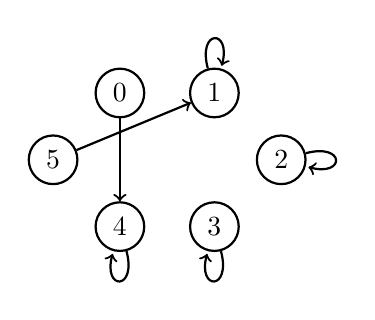
\begin{tikzpicture}[node distance={12mm}, thick, main/.style = {draw, circle}, auto=left] 
	% Sommets :
	\node[main] (0) {0}; 
	\node[main] (1) [right of=0] {1};
	\node[main] (2) [below right of=1] {2};
	\node[main] (3) [below left of=2] {3};
	\node[main] (5) [below left of=0] {5};
	\node[main] (4) [below right of=5] {4};
	% Arêtes
	\path
		(1) edge[loop above] (1)
		(2) edge[loop right] (2)
		(3) edge[loop below] (3)
		(4) edge[loop below] (4)
		(5) edge[->] (1)
		(0) edge[->] (4);
	\end{tikzpicture}
	\end{center}
\end{minipage}
\begin{minipage}{0.49\textwidth}
	\begin{center}
	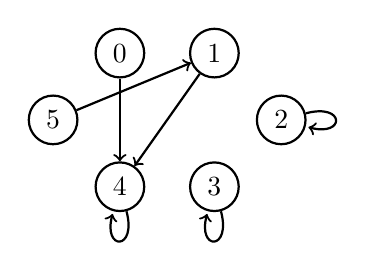
\begin{tikzpicture}[node distance={12mm}, thick, main/.style = {draw, circle}, auto=left] 
	% Sommets :
	\node[main] (0) {0}; 
	\node[main] (1) [right of=0] {1};
	\node[main] (2) [below right of=1] {2};
	\node[main] (3) [below left of=2] {3};
	\node[main] (5) [below left of=0] {5};
	\node[main] (4) [below right of=5] {4};
	% Arêtes
	\path
		(1) edge[->] (4)
		(2) edge[loop right] (2)
		(3) edge[loop below] (3)
		(4) edge[loop below] (4)
		(5) edge[->] (1)
		(0) edge[->] (4);
	\end{tikzpicture}
	\end{center}
\end{minipage}

\begin{minipage}{0.5\textwidth}
\centering \captionof{figure}{Graphe après deux unions\label{graph:uf_deux_unions_opt}}
\end{minipage}
\begin{minipage}{0.5\textwidth}
\centering \captionof{figure}{Graphe final après \textit{une} union\label{graph:uf_final_opt}}
\end{minipage}
\subsection{Implantation}
On veut représenter la fonction $\rightarrow_r$, qui associe à chaque élément de $\{0, \dots, n-1\}$ son parent dans l'arbre définit par la relation. C'est donc une fonction de $\{0, \dots, n-1\}$ dans $\{0, \dots, n-1\}$. Un tableau d'entiers convient très bien :

\begin{center}
	\includesvg[width=0.75\textwidth]{partition_tableau}
	\captionof{figure}{$T[i] = j\Leftrightarrow i\underset{graphe}{\rightarrow}j$}
\end{center}

\begin{minted}[linenos=false]{c}
struct UnionFind {
	unsigned int *parent;
	unsigned int cardinal;
	unsigned int classes_count;
};

struct UnionFind unionfind_create(unsigned int cardinal) {
	struct UnionFind uf;
	uf.repr = (unsigned int*)malloc(cardinal * sizeof(unsigned int));
	uf.cardinal = cardinal;
	for (unsigned int i = 0; i < cardinal; i++) {
		uf.parent[i] = i;
	}
	uf.classes_count = cardinal;
	return uf;
}

unsigned int unionfind_find(struct UnionFind uf, unsigned int e) {
	do {
		e = uf.parent[e];
	} while (e != uf.parent[e]); // tant que 'e' n'est pas le représentant
	return e;
}

struct UnionFind unionfind_union(struct UnionFind uf, unsigned r_a, unsigned r_b) {
	uf.parent[r_a] = r_b; // pourquoi pas... le choix est arbitraire
	uf.classes_count--;
	return uf;
}
\end{minted}
\textbf{Remarque :} le type \textit{Partition} est communément appelé \textit{UnionFind} de par le nom des deux opérations élémentaires fondamentales du type.

\textbf{Complexité temporelle :}
\begin{itemize}
	\item \textit{trouver} : Dans le pire des cas, il faut itérer sur toute la classe d'équivalence qui peut au maximum contenir tout l'ensemble, c'est-à-dire $n$ éléments. La complexité temporelle dans le pire cas est donc une fonction de $O(n)$.
	\item \textit{unir} : fonction de $O(1)$
\end{itemize}

\textbf{Reprise de l'exemple précédent :} on reprend l'ensemble $E = \{0, 1, 2, 3, 4, 5\}$ de l'exemple précédent. Le tableau des parents est au départ :
$$T = [0, 1, 2, 3, 4, 5]$$
puisque chaque élément $e$ est représentant de $\{e\}$.
\begin{itemize}
	\item Après $unir(P, 0, 4)$, on a $T = [4, 1, 2, 3, 4, 5]$
	\item Après $unir(P, 5, 1)$, on a $T = [4, 1, 2, 3, 4, 1]$
	\item On a $trouver(P, 5) = 1$ car $T[5] = 1$ puis $T[1] = 1$, donc $1$ est le représentant de $5$
	\item Après $unir(P, 5, 4) = unir(P, 1, 4)$, on a $T = [4, 4, 2, 3, 4, 1]$
	\item On a $trouver(P, 5) = 4$ car $T[5] = 1$ puis $T[1] = 4$ puis $T[4] = 4$ donc $4$ est le représentant de $5$
\end{itemize}
\subsection{Amélioration de la complexité dans le pire cas}
Les successeurs d'un représentant de classe dans le tableau forment une arborescence : 
\begin{center}
	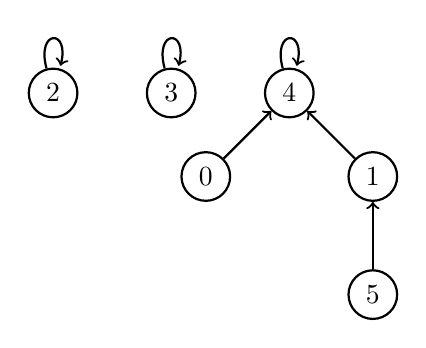
\begin{tikzpicture}[node distance={15mm}, thick, main/.style = {draw, circle}] 
		% Sommets :
		\node[main] (2) {$2$};
		\node[main] (3) [right of=2] {$3$};
		\node[main] (4) [right of=3] {$4$};
		\node[main] (0) [below left of=4] {$0$}; 
		\node[main] (1) [below right of=4] {$1$};
		\node[main] (5) [below of=1] {$5$};
		% Arêtes
		\path
		(0) edge[->] (4)
		(2) edge[loop above] (2)
		(3) edge[loop above] (3)
		(4) edge[loop above] (4)
		(5) edge[->] (1)
		(1) edge[->] (4);
	\end{tikzpicture}
	\captionof{figure}{Forêt représentative de la partition $P$ de l'exemple\label{fig:foret_partition}}
\end{center}
Si on doit parcourir toute la classe d'équivalence pour trouver le représentant, c'est que les successeurs de l'élément dont on cherche le représentant forment tout l'arbre. C'est donc une liste. L'objectif est d'éviter ce cas de figure. Si on parvient à éviter les arborescences ``filiformes'', on améliore considérablement le temps de parcours.

Dans le meilleur des cas, pour tout élément $e\in E$, on obtient le représentant de $e$ directement par \mintinline{c}{uf.parent[e]}.
\subsubsection{Union pondéré}
Prenons la partition représentée par la figure \ref{fig:foret_partition}. Supposons qu'on veuille effectuer $unir(P, 3, 4)$. On a deux possibilités :

\begin{minipage}{0.5\textwidth}
\begin{center}
	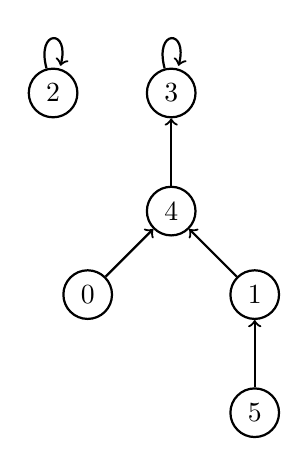
\begin{tikzpicture}[node distance={15mm}, thick, main/.style = {draw, circle}] 
		% Sommets :
		\node[main] (2) {$2$};
		\node[main] (3) [right of=2] {$3$};
		\node[main] (4) [below of=3] {$4$};
		\node[main] (0) [below left of=4] {$0$}; 
		\node[main] (1) [below right of=4] {$1$};
		\node[main] (5) [below of=1] {$5$};
		% Arêtes
		\path
		(2) edge[loop above] (2)
		(3) edge[loop above] (3)
		(4) edge[->] (3)
		(0) edge[->] (4)
		(5) edge[->] (1)
		(1) edge[->] (4);
	\end{tikzpicture}
\end{center}
\end{minipage}
\begin{minipage}{0.5\textwidth}
\begin{center}
	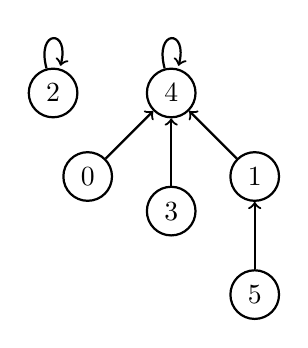
\begin{tikzpicture}[node distance={15mm}, thick, main/.style = {draw, circle}] 
		% Sommets :
		\node[main] (2) {$2$};
		\node[main] (4) [right of=2] {$4$};
		\node[main] (3) [below of=4] {$3$};
		\node[main] (0) [below left of=4] {$0$}; 
		\node[main] (1) [below right of=4] {$1$};
		\node[main] (5) [below of=1] {$5$};
		% Arêtes
		\path
		(2) edge[loop above] (2)
		(4) edge[loop above] (4)
		(3) edge[->] (4)
		(0) edge[->] (4)
		(5) edge[->] (1)
		(1) edge[->] (4);
	\end{tikzpicture}
\end{center}
\end{minipage}

\begin{minipage}{0.5\textwidth}
\centering \captionof{figure}{Choix de $3$ comme représentant}\label{fig:choix_union_3}
\end{minipage}
\begin{minipage}{0.5\textwidth}
\centering \captionof{figure}{Choix de $4$ comme représentant}\label{fig:choix_union_4}
\end{minipage}

Le second choix est optimal puisque l'arbre est moins haut. Remonter l'arbre pour trouver le représentant est moins long. Donc le critère est de choisir comme enfant l'arbre le moins haut, pour minimiser la hauteur du nouvel arbre. On ajoute donc dans \mintinline{c}{struct UnionFind} un tableau \textsf{highs}, rempli de $0$ à la création et on modifie la routine d'union par :
\begin{minted}[linenos=false]{c}
#define MAX(X, Y) (((X) < (Y)) ? (Y) : (X))

struct UnionFind unionfind_union(struct UnionFind uf, unsigned r_a, unsigned r_b) {
	if (uf.highs[r_a] > uf.highs[r_b]) {
		uf.parent[r_b] = r_a;
	} else {
		uf.parent[r_a] = r_b;
		uf.highs[r_b] = MAX(1 + uf.highs[r_a], uf.highs[r_b]);
	}
	uf.classes_count--;
	return uf;
}
\end{minted}
\textbf{Notation :} Après $i$ opérations d'unions sur la partition, on note pour tous $x\in E$ :
\begin{itemize}
	\item $t_i(x)$ le nombre d'éléments de l'arbre de racine $x$ après $i$ unions sur la partition
	\item $h_i(x)$ la hauteur de l'arbre de racine $x$ après $i$ unions sur la partition
\end{itemize}
On observe que $t_0(x) = 1$ et $h_0(x) = 0$.

$h_i(x)$ correspond à \mintinline{c}{uf.highs[x]} après $i$ opérations d'union sur la partition.

\proposition{Borne sur la hauteur} pour tout $x\in E$, pour tout $i\in \mathbb{N}$, $t_i(x)\geq 2^{h_i(x)}$.

Il s'ensuit que pour $n = Card(E)$, on a $log_2(n) \geq log_2(t_i(x))\geq h_i(x)$. La complexité temporelle dans le pire cas de $trouver$ est donc en $O(log_2(n))$.

\textbf{Démonstration :} On pose pour tout $k\in\mathbb{N}$ la proposition $P_k : \forall x\in E, t_k(x)\geq 2^{h_k(x)}$.

\underline{Initialisation :} pour $k = 0$, $t_0(x) = 2^{h_0(x)}$ car $t_0(x) = 1$ et $h_0(x) = 0$

\underline{Hérédité :} Soit $k\in\mathbb{N}$. Soient $x, y\in E$. Supposons $P_k$.

On calcul $union(P, x, y)$ :
\begin{itemize}
	\item Si $h_i(x) > h_i(y)$, alors $h_{i+1}(x) = h_i(x)$ et $t_{i+1}(x) = t_i(x) + t_i(y) \geq t_i(x) \geq 2^{h_{i}(x)} = 2^{h_{i+1}(x)}$. La hauteur et le nombre d'éléments de $y$ sont inchangés. OK.
	\item Si $h_i(x) \leq h_i(y)$, on a déjà $t_{i+1}(y) = t_i(y) + t_i(x)$. Ensuite $h_{i+1}(y) = max(h_i(y), 1 + h_i(x))$. Si $h_{i+1}(y) = h_i(y)$, tout est OK. Sinon, par l'inégalité supposée et puisque les hauteurs sont entières, on a $h_{i+1}(y) = 1 + h_i(x) = 1 + h_i(y)$. D'où $t_{i+1}(y) \geq 2^{h_i(y) + 1}\geq 2^{h_{i+1}(y)}$ . OK
\end{itemize}

\underline{Conclusion :} $(P_k)_{k\in\mathbb{N}}$ est initialisée et héréditaire, donc pour tout $k\in\mathbb{N}$, $P_k$ est vraie.
\subsubsection{Compression des chemins}
La fonction $unir$ est optimisée. On s'intéresse maintenant à optimiser $trouver$. 

Lorsqu'on parcours l'arbre pour trouver le représentant d'un élément, on peut au passage modifier cet arbre pour que tous les sommets visités par ce parcours soient ``recollés'' directement au représentant. En C, cela donne :
\begin{minted}[linenos=false]{c}
unsigned int unionfind_find(struct UnionFind uf, unsigned int e) {
// Calcul du représentant
	unsigned r = e;
	do {
		r = uf.parent[r];
	} while (r != uf.parent[r]); // tant que 'r' n'est pas le représentant
// Compression du chemin :
// on parcours à nouveau le chemin pour lier directement au représentant 'r'
	do {
		unsigned tmp = e;
		e = uf.parent[e];
		uf.parent[tmp] = r; // le sommet est lié directement au représentant
	} while (e != uf.parent[e]);
	return r;
}
\end{minted}
La première fois qu'on cherche le représentant de $e$, on double le nombre d'opérations effectués, pour effectuer la compression. Cependant, toutes les prochaines opérations $trouver$ sur les éléments du chemin seront beaucoup plus rapide. C'est donc une optimisation au niveau global.
\subsection{Exercices}
\exercise{P'tite démo de caractérisation}{10} Démontrer la proposition \refproposition{Terminaison de l'opération ``trouver''}.
% \textbf{Démonstration :} Soit $e\in C$. Il existe un unique chemin $\gamma$ de $e$ vers $r_C$ dont les sommets intérieurs sont différents de $r_C$.
% \begin{itemize}
% 	\item $(\Rightarrow)$ Supposons $e\rightarrow_r e$. Si $e\neq r_C$, alors le chemin $e\rightarrow_r e\underset{\gamma}{\rightarrow_r} r_C$ est un deuxième chemin de $e$ vers $r_C$ dont l'intérieur est privé de $r_C$, absurde.
% 	\item $(\Leftarrow)$ Supposons $e = r_C$, on a nécessairement $\gamma$ vide. Donc $e\rightarrow_r r_C = e$.
% \end{itemize}

\exercise{Affichage d'une partition}{16} Écrire une procédure :
\begin{center}
\mintinline{c}{void unionfind_display(struct UnionFind uf, char* buffer);}
\end{center}
qui affiche la partition dans un tampon \textit{buffer} grâce à la fonction \mintinline{c}{sprintf} du module \textit{stdlib} de la bibliothèque standard.\newline
\textit{\underline{Note :} on pourra utiliser la commande ``man sprintf'' dans un terminal Linux pour lire la documentation de la fonction.}

\exercise{Labyrinthe, monstres et trésors}{} On s'intéresse à la génération et à l'exploration de labyrinthes parfaits selon différentes méthodes\footnote{Inspiré librement d'un sujet X-ENS d'informatique.}.

\end{document}